
\documentclass{article}
\usepackage{graphicx}

\begin{document}
\title{Spécifiation des exigences du modèle : Jalon 2}

\author{Louis-Vincent CAPELLI \and Alexandre THEISSE \and Tom SARTORI \and Raphaël TURCOTTE}
\date{\today}
\maketitle
\newpage

\tableofcontents
\newpage

\section{Introduction}
\subsection*{Objet et portée du document}
Ce document a pour but de spécifier les exigences du jalon 2 du projet "Système
de surveillance de la qualité de l'air" (SSQA). Il est destiné aux membres du 
groupe de travail, afin de leur permettre de cerner correctement les besoins
du client et de les retranscrire lors de la conception.

\section{Présentation}
\subsection{Mise en contexte}
Lors du jalon 1, le schéma préliminaire de la base de données a été
modifié afin de mieux correspondre aux besoins du client. Le schéma résultant
est présenté ci-dessous.

\begin{figure}[h]
\centering
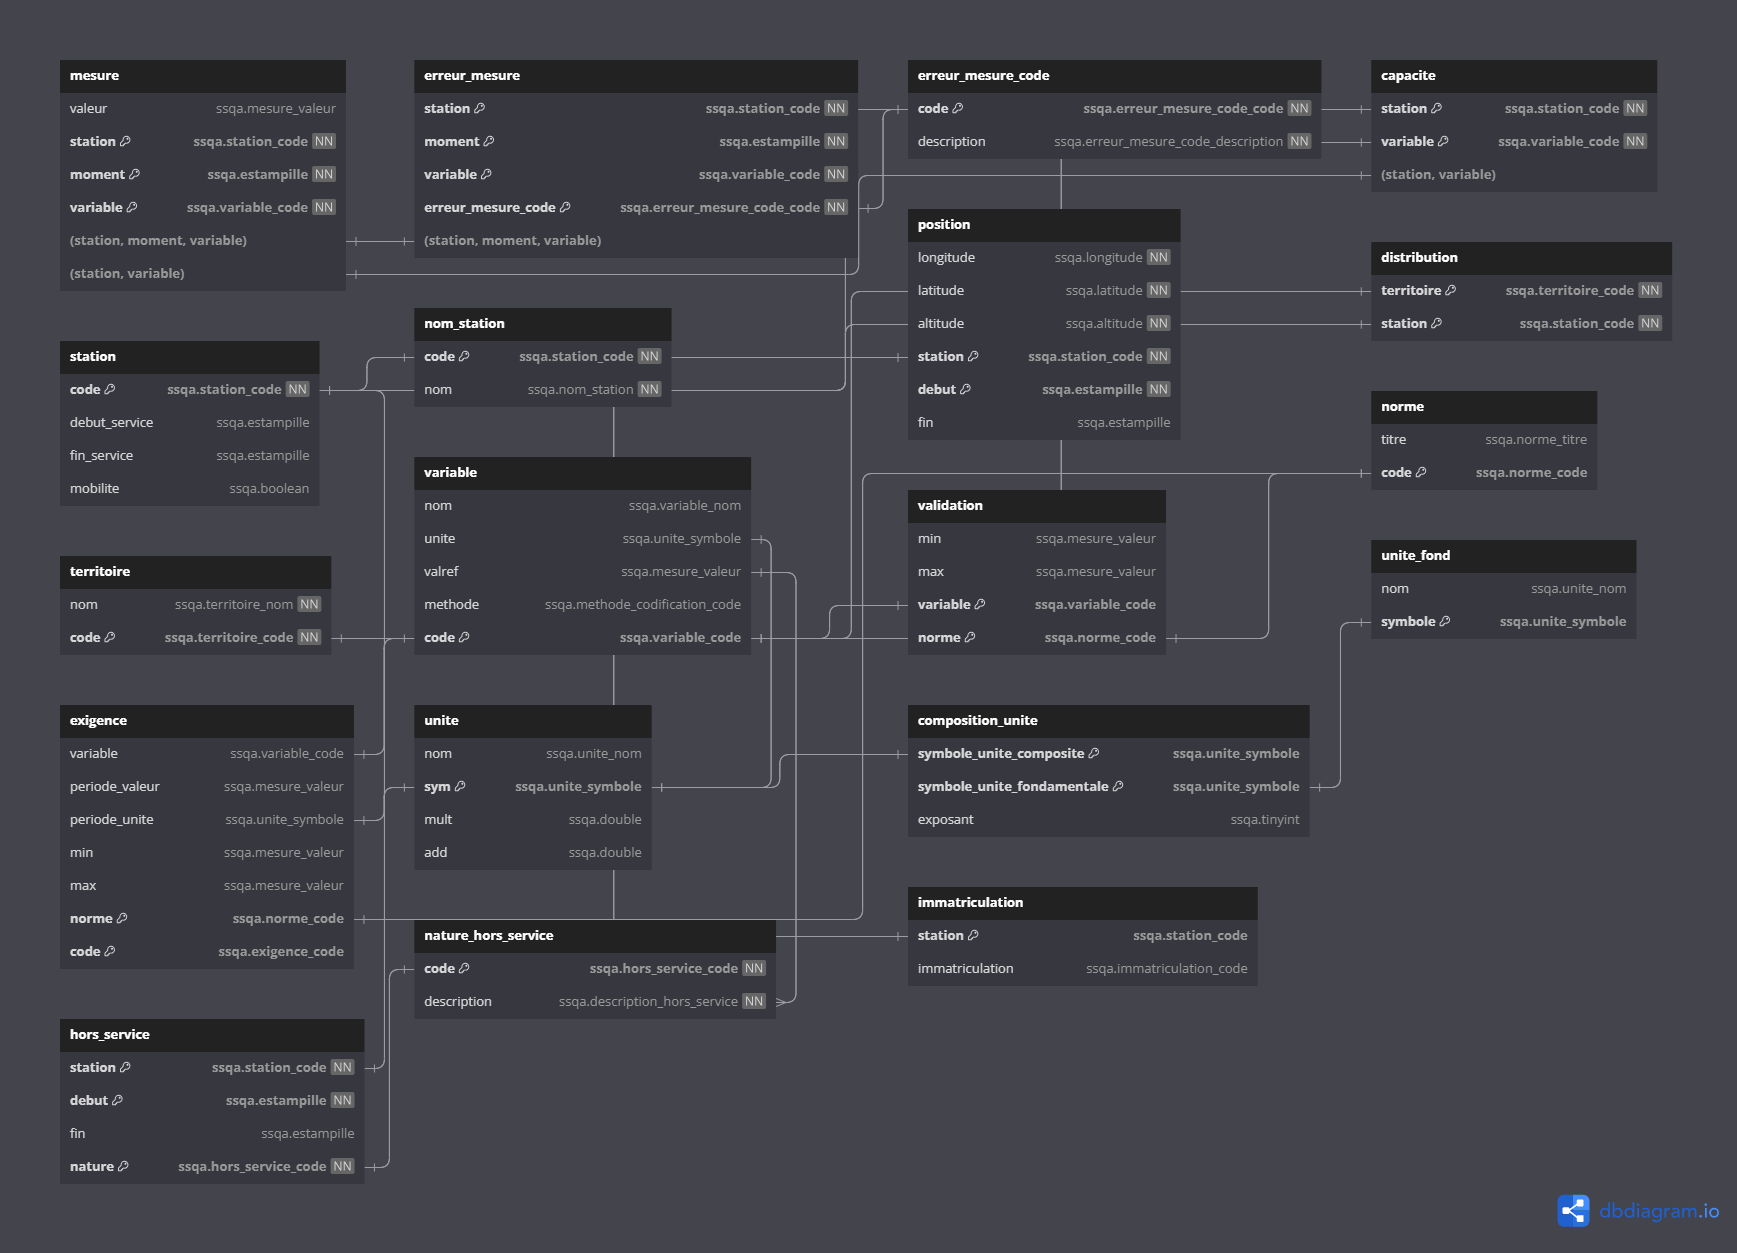
\includegraphics[scale=0.24]{modif.png}
\caption{Schéma modifié de la base de données}
\end{figure}

\subsection{Système existant}
Le système existant est une base de données PostgreSQL correspondante
au schéma modifié ci-dessus. Les scripts de création de la base de données préliminaire
ont été fournis par le client et nous y avons ajouté des scripts qui
permettent la modification de la base de données en cours d'exploitation.

\section{Problème}
Ce jalon porte sur la conception d'une API comportant les primitives
fondamentales d'évaluation, de modification, d'insertion et de retrait 
(ÉMIR) ainsi que quelques fonctions plus complexes qui illustrent
des cas d'utilisation typiques par le client.

La portée de ce jalon est restreinte aux tables Territoire, Station,
Variable et Mesure. Les tables Distribution et Capacite pourront éventuellemnt
être traitées égalemement au vu de leur proximité avec les quatre tables
citées précédemment.

\section{Exigences fonctionnelles}
\subsection{Primitives fondamentales}
\paragraph{Description} Implémenter les primitives fondamentales d'ÉMIR
pour les tables Territoire, Station, Variable et Mesure.

\subsection{Requête 1}
\paragraph{Description} Créer une fonction permet à l'utilisateur
d'effectuer la requête suivante : "Quel est l'IQA découlant des mesures
prises par la station du quartier universitaire de la ville de Sherbrooke,
le 2016-06-12 ?"

\subsection{Requête 2}
\paragraph{Description} Créer une fonction permet à l'utilisateur
d'effectuer la requête suivante : "Quelles sont les stations du territoire
de la ville de Sherbrooke ?"

\subsection{Requête 3}
\paragraph{Description} Créer une fonction permet à l'utilisateur
d'effectuer la requête suivante : "Quels sont les quartiers de la ville
de Sherbrooke qui dépassent la norme canadienne de la qualité de l'air
au moins n fois par année ?"

\subsection{Requête 4}
\paragraph{Description} Créer une fonction permet à l'utilisateur
d'effectuer la requête suivante : "Dans un territoire donné, au cours de
l'année 2021, quels sont les polluants qui ont dépassé la valeur de 
référence d'au moins 10\% ?"

\subsection{Requête 5}
\paragraph{Description} Créer une fonction permet à l'utilisateur
d'effectuer la requête suivante : "Quels sont les territoires ayant au
moins trois fois par mois un mauvais IQA au  cours des deux dernières
années ?"

\end{document}
